%%%%%%%%%%%%%%%%%%%%%%%%%%%%%%%%%%%%%%%%%%%%%%%%%%%%%%%
%                File: OpEx_temp.tex                  %
%             Created: 2 September 2009               %
%                Updated: 15 May 2015                 %
%                                                     %
%           LaTeX template file for use with          %
%           OSA's journals Optics Express,            %
%             Biomedical Optics Express,              %
%            and Optical Materials Express            %
%                                                     %
%  send comments to Theresa Miller, tmiller@osa.org   %
%                                                     %
% This file requires style file, opex3.sty, under     %
%              the LaTeX article class                %
%                                                     %
%   \documentclass[10pt,letterpaper]{article}         %
%   \usepackage{opex3}                                %
%                                                     %
%                                                     %
%       (c) 2015 Optical Society of America           %
%%%%%%%%%%%%%%%%%%%%%%%%%%%%%%%%%%%%%%%%%%%%%%%%%%%%%%%

%%%%%%%%%%%%%%%%%%%%%%% preamble %%%%%%%%%%%%%%%%%%%%%%%%%%%
\documentclass[10pt,letterpaper]{article}
\usepackage{opex3}
\usepackage{color}
\usepackage[latin9]{inputenc}
\usepackage{mathrsfs,amsmath}
\usepackage{graphicx}%
\usepackage{float}
\usepackage{amsfonts}%
\usepackage[titletoc]{appendix}
\usepackage{amssymb}
\usepackage{braket}
\usepackage{bm}
\newcommand{\mb}[1]{\bm{#1}}
\usepackage[T1]{fontenc}



\def\Nabla{\bm{\nabla}}
\def\bm{\mathbf}
\def\curl{\Nabla\times}
\def\div{\Nabla\cdot}
\def\lap{\Delta}
\def\vlap{\Delta}
\def\x{\hat{e}_{x}}
\def\y{\hat{e}_{y}}
\def\z{\hat{e}_{z}}
\def\p{\partial}
\DeclareMathOperator{\Tr}{Tr}
\bibliographystyle{ieeetr}
%%%%%%%%%%%%%%%%%%%%%%% begin %%%%%%%%%%%%%%%%%%%%%%%%%%%%%%
\begin{document}

%%%%%%%%%%%%%%%%%% title page information %%%%%%%%%%%%%%%%%%
\title{Title goes here}

\author{Petar Tzenov$^{1,*}$,  David Burghoff$^{2}$, Qing Hu$^{2}$ and Christian Jirauschek$^1$}

\address{$^1$ Institute for Nanoelectronics, Technical University f Munich, D-80333 Munich, Germany}
\address{$^2$ Department of Electrical Engineering and Computer Science, Research Laboratory of Electronics, Massachusetts Institute of Technology, Cambridge,
	Massachusetts 02139, USA}

\email{$^*$petar.tzenov@tum.de} %% email address is required

% \homepage{http:...} %% author's URL, if desired

%%%%%%%%%%%%%%%%%%% abstract and OCIS codes %%%%%%%%%%%%%%%%
%% [use \begin{abstract*}...\end{abstract*} if exempt from copyright]

\begin{abstract}
 The generation of frequency combs in the mid-infrared and terahertz from compact and potentially cheap sources could have a strong impact on spectroscopy as many molecules have their ro-vibrational bands in this spectral range. Quantum cascade lasers (QCLs) are the perfect candidates for comb generation in the mid- and far-infrared portions of the electromagnetic spectrum, due to the broadband nature of their gain as well as their high quantum efficiency. Here we present a theoretical model based on a full numerical solution of  Maxwell-Bloch equations suitable for the simulation of such devices, as we attempt to identify the main ingredients for a successful generation of QCL based terahertz combs. We show that our approach captures the intricate interplay between four wave mixing, spatial hole burning and chromatic dispersion that are essentially present in free running QCLs and come to conclusions regarding comb like and chaotic regimes of multimode operations reported in these type of devices. 
\end{abstract}

\ocis{(000.0000) General.} 

%%%%%%%%%%%%%%%%%%%%%%% References %%%%%%%%%%%%%%%%%%%%%%%%%
\bibliography{literature}

%%%%%%%%%%%%%%%%%%%%%%%%%%  body  %%%%%%%%%%%%%%%%%%%%%%%%%%
\section{Introduction}
\label{sec:intro}

Quantum cascade lasers (QCLs)  promise to be efficient, cheap and compact generators of frequency combs in the mid- and far- infrared portions of the electromagnetic spectrum. QCL based combs in both spectral regions have been previously demonstrated \cite{burghoff2014terahertz,hugi2012mid}, but due to material dispersion or optical instabilities their spectral coverage has remained just a fraction of their central frequency. Thus the development of an octave spanning frequency comb is still out of reach [Cite Faist paper and why would octave comb be attractive]. 

The most obvious method to generate multiple, evenly spaced longitudinal modes is active mode locking (AML) via radio frequency (RF) modulation of the injection current or the applied bias. AML for quantum cascade lasers has proven to be elusive and only limited success has been achieved so far \cite{wang2009mode,wang2015generating}. It was widely believed that this is due to the QCL's inherent ultrafast gain recovery time, which broadens an incident pulse's time profile as if it propagates through a saturable gain material. In fact, this understanding has been partially defeated, as it has been suggested by simulations \cite{wang2015active} that picosecond pulses \emph{can} be produced in  QCLs with short gain recovery by opening a brief net gain window via amplitude modulation of the bias field in only a short section of the cavity. Furthermore, latest experimental results \cite{wang2015generating} also show successful AML in combination with injection seeding for a fast gain recovery ($\approx 5$ ps) terahertz QCL based on LO phonon design, where the authors have stressed on the importance to consider waveguide effects within the design parameters.  

On the other hand, active mode locking is only a sufficient, but not a necessary condition for the generation of stable frequency combs. Indeed, experimental results have shown comb generation in the mid-infrared \cite{hugi2012mid} as well as, more recently, the terahertz \cite{burghoff2014terahertz,rosch2015octave} [CITE BERLIN] range based on free running QCLs. High order nonlinear optical processes, such as four wave mixing, are the main mode proliferation mechanisms that contribute to comb formation \cite{khurgin2014coherent} [VILLARES]. In contrast, it has been argued that group velocity dispersion (GVD) is the thorn in the design of frequency combs as it leads to pulse broadening and limits the full exploitation of the gain bandwidth of the material [REFERENCES]. In the terahertz regime, the two widest comb generating devices demonstrated so far \cite{burghoff2014terahertz,rosch2015octave}, have shown a strong variation of the beatnote's linewidth with changing injection current and thus indicate that "comb"  operation regimes are only a fraction of the whole dynamic range of these lasers. 

This paper addresses the reasons behind the alternation between comb and non-comb regimes of multimode operation in free running THz QCLs. In Sec. \ref{sec:thmodel} we present our theoretical model based on a full numerical solution of the semiclassical Maxwell-Bloch equations, where a single optical and a single resonant tunneling transition have been coherently included. Despite the existence of numerous implementations of the Maxwell-Bloch equations for simulation of QCLs \cite{callebaut2005importance,wang2015active,dupont2010simplified} [CITE MORE], to the extend of our knowledge, we are the first authors to demonstrate transient dynamic simulations of QCL comb operation. In Sec. \ref{subsec:numthztds}, we stress on the implications of the inclusion of the resonant tunneling effect onto the system dynamics. Namely, the incorporation of a strong non-radiative coupling between injector and upper laser level of a single QCL module induces a noticeable splitting of the optical spectra, as experimentally observed in Ref. \cite{burghoff2014terahertz}. Furthermore, we can deduce a non-trivial GVD relation governing the propagation of light near those resonances. We continue our discussion, in Sec. \ref{subsec:FWM}, by investigating via numerical experiments the dominant mode proliferation mechanisms captured by our model. From our results we can clearly confirm that degenerate four wave mixing, and more specifically third-order difference frequency generation, is the main effect contributing to multimode emission, as we investigate conditions to set off this nonlinear process. Lastly, in Sec. \ref{subsec:tdsims} we study the chaotic beatnote regime of operation in multimode QCLs as a form of multi-pulse behaviour in lasers with strong chromatic dispersion. 

\section{Theoretical Model}
\label{sec:thmodel}

The Maxwell-Bloch (MB) equations are a semi-classical model describing the light-matter interaction in microscopic systems, where the coherent coupling between the optical field and the gain medium is treated within a density matrix formalism, whereas the effect of the induced polarization onto the propagating optical field is captured via the classical Maxwell's equations. This model is a generalization of the rate equations approach, which allows us to include optical nonlinearities and quantum coherence effects into electron transport simulations and thus incorporate the physics of four wave mixing and resonant tunneling into the system dynamics. We start with a derivation of the Maxwell-Bloch equations for a three level system with a resonant tunneling transition and an optical transition. Then, we employ the rotating wave and slowly varying envelope approximations to obtain a closed set of equations, describing the temporal evolution of the density matrix as well as the electric field envelope. These two approximations provide us with the added benefit that they are less restrictive on the chosen time step and grid size, which allows us to perform our simulations over many thousands of round trips in a reasonable amount of time. Last but not least, we include the contributions of various nonradiative scattering mechanisms to the carrier dynamics, via a  rate equations approach, where the corresponding rates are extracted from our ensemble Monte Carlo simulations \cite{jirauschek2014modeling} [CITE MORE].

\begin{figure}[h!]
\centering
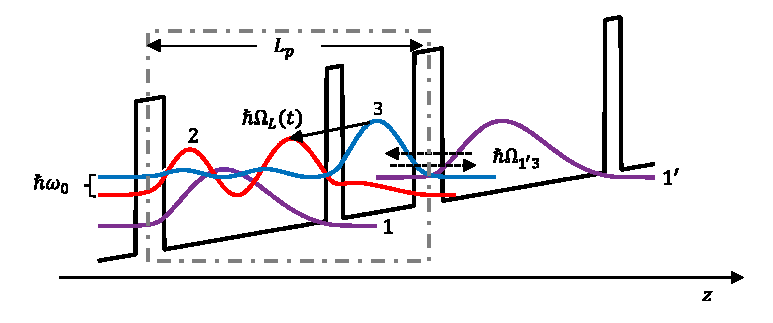
\includegraphics[scale=0.8]{img01_b.eps}
\caption{A schematic diagram of a simple three level LO-phonon THz QCL, where the upper laser level is populated via resonant tunneling.} \label{fig:img01}
\end{figure}

Let us consider a simple three level resonant phonon QCL system as depicted in Fig. \ref{fig:img01}. In this configuration, there are four relevant levels $\Ket{1'}, \Ket{3}, \Ket{2} $ and $\Ket{1}$ which are the injector level, the upper and lower laser levels and the depopulation level, respectively. $\Ket{1'}$ couples to $\Ket{3}$ via the anticrossing energy $\hbar\Omega_{1'3}$, whereas the upper and lower laser levels interact via the optical Rabi frequency $\Omega_L(t)= \mu_{32}E_z(t)/\hbar$, where $\mu_{32} = |e| \Bra{3}\hat{z} \Ket{2}$ is the dipole matrix element, for convenience taken with a positive sign, $E_z(t)$ is the electric field component along the growth direction $z$ and $|e|$ is the elementary charge. Lastly, we assume that the energy separation between $\Ket{1'}$ and $\Ket{3}$ is $\Delta_{1'3} = \hbar \epsilon$ and that between the upper and lower laser levels $\Delta_{32} = \hbar \omega_0$.
The evolution of electron wave packets, cascading through the structure, are treated quantum mechanically within the density matrix formalism, where the equation of motion (EOM) is given by the von Neumann equation:
\begin{align}
 \label{eq:vonNeumann}
\frac{d \hat{\rho}}{dt} =\frac{i}{\hbar}[\hat{\rho},\hat{H}].
\end{align}
Above $\hat{\rho}$ denotes the density operator, $\hat{H}$ the Hamiltonian of the system, and $[\cdot,\cdot]$ the usual quantum mechanical commutator. In general, $\hat{H}$ contains many different contributions corresponding to various physical mechanisms that determine the overall carrier transport in the system. These could be radiative transitions, resonant tunneling or incoherent scattering events such as LO phonon, electron-electron, interface roughness scattering and others. In view of the fact that we want to numerically solve Eq. (\ref{eq:vonNeumann}), incorporating all those effects quantum mechanically proves to be a difficult task and it is out of the scope of this research. Therefore, under the assumption of weak non-parabolicity and using that the tunneling and radiative transitions conserve the in-plane momentum, we can include those two processes fully quantum mechanically, whereas treat all incoherent scattering process within a rate equation approach \cite{iotti2005microscopic}. The rates for the latter subband transition events will not be chosen arbitrarily, but rather calculated with our well established ensemble Monte Carlo simulation code \cite{jirauschek2014modeling}. [CITE MORE] 

When resonant tunneling transitions are modelled, one usually employs the so called tight-binding approximation \cite{bastardwave}, where the wave functions are calculated for a single isolated period, whereas the electron subbands in adjacent modules are simply translated in space and energy by the module length $L_p$ \cite{callebaut2005importance}. However, the true time evolution of the system is still governed by the full, or the extended, Hamiltonian ($\hat{H}_{ext}$), consisting of multiple modules, so we need to compensate for the fact that we are using a tight-binding basis by including the correct anticrossing energies between levels spanning an intermodule barrier. In our case these are the injector and upper laser level where their coupling energy is assumed to be $\hbar \Omega_{1'3}$ (see Fig. \ref{fig:img01}). Finally, in this tight-binding basis, one can expand the von Neumann equation in matrix form as
\begin{align}
 \label{eq:vonNeumannmatrix}
& \frac{d}{dt} \begin{pmatrix}
\rho_{1'1'}& \rho_{1'3} & \rho_{1'2} \\
\rho_{31'} & \rho_{33} & \rho_{32} \\ 
\rho_{21'} & \rho_{23} & \rho_{22}
\end{pmatrix}  =   \frac{i}{\hbar}\left [
\begin{pmatrix}
\rho_{1'1'}& \rho_{1'3} & \rho_{1'2} \\
\rho_{31'} & \rho_{33} & \rho_{32} \\ 
\rho_{21'} & \rho_{23} & \rho_{22}
\end{pmatrix} , 
\overbrace{\begin{pmatrix} 
	\frac{\hbar \epsilon}{2} & \hbar\Omega_{1'3} & 0 \\
	\hbar\Omega_{1'3}  & -\frac{\hbar	\epsilon}{2} &  \hbar\Omega_{L}(t) \\
	0  &\hbar\Omega_{L}(t) & -\frac{\hbar \epsilon}{2}-\hbar\omega_{0}   
	\end{pmatrix} }^{\text{resonant tunneling and radiative coupling}}
\right ]  \nonumber \\
& + 
\underbrace{\begin{pmatrix}
	-\frac{\rho_{1'1'}}{\tau_{1'}} + (\frac{1}{\tau_{31'}}+\frac{1}{\tau_{31}})\rho_{33}  +  (\frac{1}{\tau_{21'}}+\frac{1}{\tau_{21}})\rho_{22} & \tau_{\parallel 1'3}^{-1}\rho_{1'3} & \tau_{\parallel 1'2}^{-1}\rho_{1'2}\\
   \tau_{\parallel 1'3}^{-1}\rho_{31'} & \frac{\rho_{1'1'}}{\tau_{1'3}}   - \frac{\rho_{33}}{\tau_{3}} +  \frac{\rho_{22}}{\tau_{23}} &  \tau_{\parallel 32}^{-1}\rho_{32}\\
   \tau_{\parallel 1'2}^{-1}\rho_{21'}& \tau_{\parallel 32}^{-1}\rho_{32} &	\frac{ \rho_{1'1'}}{\tau_{1'2}} + \frac{\rho_{33} }{\tau_{32}} 	- \frac{\rho_{22}}{\tau_2}
\end{pmatrix}}_{\text{scattering rates matrix}},
\end{align}
where $\rho_{i,j} = \Bra{i} \hat{\rho} \Ket{j}$ are the corresponding density matrix elements and we have set the zero energy at $E_0 = (E_{1'}+E_{3})/2 $. Furthermore $\tau_{ij}^{-1}$ denotes the total outscattering rate from level $i$ to level $j$, $\tau_{i}$ is the lifetime of level $i$ and
$$
	\tau_{\parallel ij}^{-1} = \frac{1}{2}(\frac{1}{\tau_{i}} +\frac{1}{\tau_{j}}) + \frac{1}{\tau_{pure}}   
$$
is the damping rate of the coherence between levels $i$ and $j$, containing lifetime broadening and other "pure" dephasing mechanisms, which scramble the phase coherence between these subbands [CITE MORE]. 

Notice that in Eq. (\ref{eq:vonNeumannmatrix}) we have omitted the time evolution related to state $\Ket{1}$. This is due to the fact that the depopulation level, $\Ket{1}$, is effectively the injector level of the next period, which allows us to eliminate it from the model by employing "periodic" boundary conditions in the scattering rates matrix. It is vital for the simulation that these periodic boundary conditions are implemented correctly. This is so, because our model is formulated in a manner which does not phenomenologically include the injection current density $J$ into the equations. Instead, we assume a periodic system where all carriers that reach the depopulation level $\Ket{1}$ are immediately re-injected into the system through level $\Ket{1'}$. In such a configuration the overall carrier density has to be conserved, which means that the relation $\sum_{j} d \rho_{jj}/dt =0 $ has to be satisfied at all times. Then, the current injected into the system is essentially equal to the current entering into the depopulation level, $\Ket{1}$. From rate equation analysis, the current through a system with average carrier concentration $N$, is given by the formula
\begin{equation}
\label{eq:currentdensity}
J = e N L_p  \left( \frac{\rho_{33}}{\tau_{31}} + \frac{\rho_{22}}{\tau_{21}} + \frac{\rho_{1'1'}}{\tau_{1'1}} \right)\approx e N L_p \left( \frac{\rho_{33}}{\tau_{31}} + \frac{\rho_{22}}{\tau_{21}}  \right),  
\end{equation}
with the approximation obtained by assuming a negligible scattering rate $1/\tau_{1'1}$. Note that this expression is similar to the one in \cite{kumar2009coherence}, however it could be easily generalized for arbitrary number of, say M, levels via
\begin{equation}
J = e N  L_p \left( \sum_{j=2}^{M}\frac{\rho_{jj}}{\tau_{j1}} + \frac{\rho_{1'1'}}{\tau_{1'1}} \right),
\end{equation}
where $\rho_{1'1'}$ denotes the injector level element and the $\rho_{jj}$ the density matrix elements corresponding to all electron transport "channel" levels within a single module.   

Since the density matrix is Hermitian, Eq. (\ref{eq:vonNeumannmatrix}) boils down to a system of six coupled ordinary differential equations for the unknowns $\rho_{1'1'}, \rho_{33},\rho_{22},\rho_{1'3},\rho_{32} $ and $\rho_{1'2}$. 

The coupling of the microscopic density matrix equations to the macroscopic Maxwell's equations is usually done via the incorporation of  polarization term in Maxwell's equations as the expectation value of the quantum mechanical dipole moment operator,
\begin{equation} 
P_z = -N\Gamma \Tr\{\rho \mu\} = -N\Gamma(\mu_{32}\rho_{32} + \mu_{23}\rho_{23}) =  -N\Gamma\mu_{32}(\rho_{32}+\rho_{23}) , \label{eq:fullpolarization}
\end{equation}
where $\Gamma$ is the spatial overlap factor between the optical field  and the active region. The negative sign in the above expression is due to the fact that we have taken the dipole element as $|e| \Bra{3}\hat{z} \Ket{2}$ instead of$-|e| \Bra{3}\hat{z} \Ket{2}$. Assuming no free electric charges and also weak inhomogeneities in the polarization field, we obtain the classical wave equation for  $E_z$:
\begin{equation}
\Big (\partial^2_{x} -\frac{n^2}{c^2}\partial^2_{t} \Big) E_z = \frac{1}{\epsilon_0 c^2}\partial^2_t P_z, 
\label{eq:fullwave}
\end{equation}
where $x$ denotes the propagation direction, $c$ the speed of light in vacuum, $n$ is the refractive index of our material and $\epsilon_0$ is the permittivity of free space.

\subsection{Maxwell-Bloch equations for a Fabry-Perot resonator} 
\label{subsec:mbforfpresonator}
 Let us consider a Fabry-Perot resonator of a certain length $L$, and employ the rotating wave (RWA) and the slowly varying envelope approximations (SVEA) \cite{boyd2003nonlinear,gordon2008multimode}. The optical field inside the cavity can be written as a superposition of forward and backward propagating waves
\begin{align}
	E_z(x,t) &= \frac{1}{2} \big [ f_{+}(x,t) e^{i(k_c x-\omega_c t)} + f_{-}(x,t) e^{-i(k_c x+\omega_c t)} + c.c \big],\label{eq:e-ansatz}
\end{align}
where "c.c." denotes the complex conjugate of the preceding expression, the $+$ and $-$ signs specify the forward/backward propagating waves' envelopes, respectively, and $\omega_c$  and $k_c$ are the field's  carrier frequency and wave number, related by $k_c = n \omega_c  / c$. Since the superposition of two counter propagating waves forms a standing wave, this will lead to the formation of an inversion grating along the propagation direction $x$, a phenomenon also known as spatial hole burning. Thus for the diagonal elements of the density matrix we make the following ansatz:
\begin{align}
      \rho_{ii}(x,t) = \rho_{ii}^0(x,t) + \rho_{ii}^+(x,t) e^{2ik_c x} + \rho_{ii}^-(x,t)e^{-2ik_c x}, \label{eq:ii-ansatz}
\end{align}
where $\rho_{ii}^+ = (\rho_{ii}^-)^*$ are the inversion grating's amplitudes [CITE MORE]. The ansatz in Eq. (\ref{eq:ii-ansatz}) is justified since the population inversion follows the \emph{intensity} of the field and not its amplitude, from where it follows that the inversion grating ought to be proportional to $\propto sin(2k_cx)$ and not $sin(k_c x)$. Lastly, we decompose the coherences of the density matrix as
\begin{subequations}
	\label{eq:cohansatz}
\begin{align}
   \rho_{32}(x,t) &= \eta_{32}^{+}(x,t)e^{i(k_cx-\omega_ct)} + \eta_{32}^{-}(x,t)e^{-i(k_c x+\omega_c t)}, \label{eq:32ansatz} \\
   \rho_{1'2}(x,t) &= \eta_{1'2}^{+}(x,t)e^{i(k_c x - \omega_c t)} + \eta_{1'2}^{-}(x,t)e^{-i(k_c x+\omega_c t)}, \label{eq:12ansatz} \\
   \rho_{1'3}(x,t) &= \rho_{1'3}^0(x,t) + \rho_{1'3}^{+}(x,t) e^{2ik_cx} +  \rho_{1'3}^{-}(x,t) e^{-2ik_cx}.   \label{eq:13ansatz}
\end{align}
\end{subequations}
Notice that the term $\rho_{1'3}$ is assumed to evolve in a similar manner as the $\rho_{jj}$'s whereas $\rho_{32}$ and $\rho_{1'2}$ follow the electric field ansatz. Indeed, taking Eqs. (\ref{eq:e-ansatz}) and (\ref{eq:12ansatz}) and inserting into the product $E\rho_{1'2}$ of Eq. (\ref{eq:DMrho13}), after applying the rotating wave approximation we get
$$
E\rho_{1'2} \approx  \frac{1}{2}\big (f_{+}^*\eta_{1'2}^{+}+f_{-}^*\eta_{1'2}^{-} + f_{-}^* \eta_{1'2}^{+}e^{2ik_c x} +f_{+}^* \eta_{1'2}^{-}e^{-2ik_c x}  \big ),
$$
which does not contain terms oscillating with $e^{\pm i\omega_ct }$, and hence confirms that within the rotating wave approximation the spatio-temporal dependence of $\rho_{1'3}$ can be assumed to follow Eq. (\ref{eq:13ansatz}).

Finally, plugging Eqs. (\ref{eq:e-ansatz}), (\ref{eq:ii-ansatz}) and (\ref{eq:cohansatz}) into Eqs. (\ref{eq:vonNeumannmatrix}), (\ref{eq:fullpolarization}) and (\ref{eq:fullwave})  and invoking the rotating wave and slowly varying amplitude approximations, we obtain our model in its final form
\begin{subequations}
	\label{eq:finalthreelevelmodel}
\begin{align}
&\frac{n}{c}\partial_t f_{\pm} \pm \partial_{x}f_{\pm} = -i\frac{N \Gamma \mu_{32} k_c}{\epsilon_0 n^2} \eta_{32}^{\pm} - l_0 f_{\pm} \label{eq:rtwave} .\\
&\frac{d \rho_{1'1'}}{d t}^{0} = i\Omega_{1'3} (\rho_{1'3}^{0} - \rho_{31'}^{0}) + (\frac{1}{\tau_{31'}} + \frac{1}{\tau_{31}})\rho_{33}^{0} 
 + (\frac{1}{\tau_{21'}} + \frac{1}{\tau_{21}})\rho_{22}^{0} - \frac{\rho_{1'1'}^{0}}{\tau_{1'}} \label{eq:rho11-dm} \\
&\frac{d \rho_{1'1'}}{d t}^{\pm} = i\Omega_{1'3} (\rho_{1'3}^{\pm} - \rho_{31'}^{\pm}) + (\frac{1}{\tau_{31'}} + \frac{1}{\tau_{31}})\rho_{33}^{\pm}  
+ (\frac{1}{\tau_{21'}} + \frac{1}{\tau_{21}})\rho_{22}^{\pm} - (\frac{1}{\tau_{1'}} + 4k_c^2D )\rho_{1'1'}^{\pm}  \label{eq:rtpop1grating}\\
&\frac{d \rho_{33}}{d t}^0 = i\Omega_{1'3} (\rho_{31'}^0 - \rho_{1'3}^0) + i\frac{\mu_{32}}{2\hbar} \big (f_{-}^*\eta_{32}^{-}+f_{+}^*\eta_{32}^{+} - c.c. \big )+ \frac{1}{\tau_{1'3}}\rho_{1'1'}^0 +  \frac{1}{\tau_{23}}\rho_{22}^0 - \frac{\rho_{33}^0}{\tau_{3}}  \\
&\frac{d \rho_{33}}{d t}^{+}   = i\Omega_{1'3} (\rho_{31'}^{+} - \rho_{1'3}^{+}) + i\frac{\mu_{32}}{2\hbar}\big ( f_{-}^*\eta_{32}^{+}-f_{+}(\eta_{32}^{-})^* \big ) 
+ \frac{\rho_{1'1'}^+}{\tau_{1'3}} +  \frac{\rho_{22}^+}{\tau_{23}} - (\frac{1}{\tau_{3}} +4k_c^2D) \rho_{33}^+ \label{eq:rtpop3grating}\\
&\frac{d \rho_{22}}{d t}^{0}  = -i\frac{\mu_{32}}{2\hbar} \big (f_{-}^*\eta_{32}^{-}+f_{+}^*\eta_{32}^{+} - c.c. \big ) + \frac{1}{\tau_{1'2}}\rho_{1'1'}^0  +  \frac{1}{\tau_{32}}\rho_{33}^{0} - \frac{\rho_{22}^0}{\tau_{21}} , \\
&\frac{d \rho_{22}}{d t}^{+}   = - i\frac{\mu_{32}}{2\hbar}\big ( f_{-}^*\eta_{32}^{+}-f_{+}(\eta_{32}^{-})^* \big )  + \frac{1}{\tau_{1'2}}\rho_{1'1'}^+  +  \frac{1}{\tau_{32}}\rho_{33}^+ - (\frac{1}{\tau_{2}}+4k_c^2D) \rho_{22}^+ , \label{eq:rtpop2grating}\\
&\frac{d \rho_{1'3}}{d t}^0  = -i\epsilon\rho_{1'3}^0 +i \Omega_{1'3}(\rho_{1'1'}^{0} - \rho_{33}^{0}) +i\frac{\mu_{32}}{2 \hbar}\big (f_{+}^*\eta_{1'2}^{+}+f_{-}^*\eta_{1'2}^{-} \big ) -
\tau_{\parallel 1'3}^{-1} \rho_{1'3}^{0} ,  \\
&\frac{d \rho_{1'3}}{d t} ^\pm = -i\epsilon\rho_{1'3}^\pm  +i\Omega_{1'3}(\rho_{1'1'}^{\pm} - \rho_{33}^{\pm}) +i \frac{\mu_{32}}{2 \hbar} f_{\mp}^* \eta_{1'2}^{\pm} 
- (\tau_{\parallel 1'3}^{-1} +4k_c^2 D)\rho_{1'3}^{\pm} ,\label{eq:rho13grating}\\
&\frac{d \eta_{32}^{\pm}}{d t}   = i(\omega_c - \omega_{0})\eta_{32}^{\pm} +i \frac{\mu_{32}}{2\hbar}\Big(  f_{\pm}(\rho_{33}^0-\rho_{22}^0) + f_{\mp}(\rho_{33}^\pm-\rho_{22}^\pm) \Big ) - i\Omega_{1'3}\eta_{1'2}^{\pm}
- \tau_{\parallel 32}^{-1}\eta_{32}^\pm , \\
&\frac{d \eta_{1'2}^\pm}{d t}  = i(\omega_c - \omega_{0}-\epsilon)\eta_{1'2}^{\pm} +i \frac{\mu_{32}}{2\hbar}(f_{\pm }\rho_{1'3}^0 + f_{\mp} \rho_{1'3}^{\pm}) - i\Omega_{1'3}\eta_{32}^{\pm} - \tau_{\parallel 1'2}^{-1}\eta_{1'2}^\pm.\label{eq:rho12-dm}
\end{align}
\end{subequations}
Notice that in Eq. (\ref{eq:rtwave}) we have added, phenomenologically, a linear amplitude loss coefficient $l_0$, and in equations (\ref{eq:rtpop1grating},\ref{eq:rtpop3grating} ,{\ref{eq:rtpop2grating},\ref{eq:rho13grating}) a diffusion term $4k_c^2D$ describing the diffusion rate at which carriers diffuse away from peaks of the population grating. Here $D$ denotes the diffusion constant, which for GaAs-AlGaAs systems is 46 cm$^2$/sec \cite{wang2009mode}.
 
\section{Applications}
\label{sec:application}
\subsection{Self-consistent simulations of LO-phonon terahertz QCLs}
\label{subsec:extension}
In this section we apply our model to simulate one of the best performing QCL based terahertz frequency combs so far, the QCL design in \cite{burghoff2014terahertz}. This laser is based on a resonant LO phonon active region, lasing at the central frequency  $f_0\approx 3.5$ THz, and  has been shown to produce a stable multimode spectrum containing more than 70 equidistant longitudinal modes in a free running regime of operation. At optimal biases, field autocorrelation measurements show a broadband periodic signal with a very strong and narrow beatnote with minimal reported FWHM linewidth of approximately 1.53 kHz. Furthermore, a novel comb coherence detection technique, SWIFT \cite{burghoff2015evaluating}, was used to prove the stability of the terahertz comb over a large number of round trips. 
To correctly describe the device under test, we start off by wave function calculations in order to determine operating regimes where the "single resonant tunneling and single optical transition" assumption of our model is justified. For these values of the bias, in Sec. \ref{subsec:numthztds}, we conduct numerical experiments to calculate the spectrally resolved complex refractive index as well as to investigate the gain dispersion of the device in question. In Sec. \ref{subsec:FWM} we confirm \cite{khurgin2014coherent} that degenerate four wave mixing, and more specifically third order difference frequency generation, is the dominant multimode mechanism and we also discuss favourable conditions for this process to occur. Finally, in Sec. \ref{subsec:tdsims} we present results from long time simulations of this device and show the onset of different steady state regimes, similar to what can be observed in experiment.

\begin{figure}[h!]
	\begin{center}
		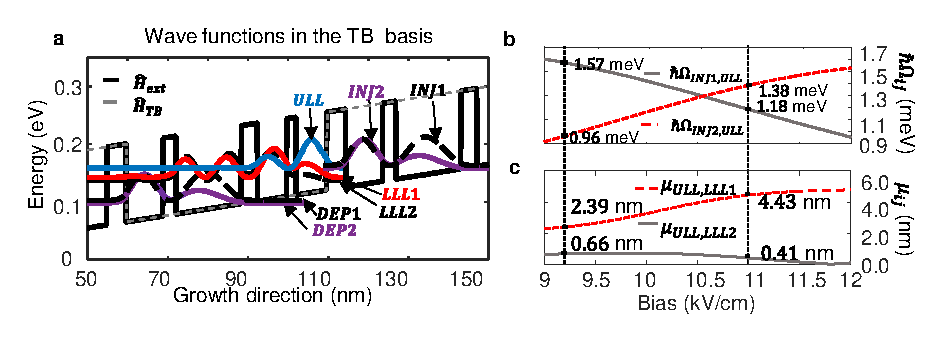
\includegraphics[scale=.85]{img02_b.eps}
		\caption{\textbf{a}, The moduli squared of the wave functions of the THz QCL in Ref. \cite{burghoff2014terahertz} within the tight-binding approximation. \textbf{b}, The anticrossing coupling strengths between the pair of injector levels, $\ket{INJ1},\ket{INJ2}$, and the upper laser level $\ket{ULL}$, computed via the method in \cite{bastardwave}. \textbf{c}, Dipole elements calculated for the same laser, obtained with the extended basis Hamiltonian, $\hat{H}_{ext}$.} \label{fig:img02}
	\end{center}	
\end{figure}

Fig. \ref{fig:img02}a illustrates the calculated wave functions at bias of 11 kV/cm obtained with the tight binding approximation. From graphical inspection we see that there are in total of five relevant levels per period, which we will refer to, according to their assumed role, as $\Ket{ULL}$ for the upper laser level, $\Ket{LLL1}$ for the higher energy level from a pair of lower laser levels, $\Ket{LLL2}$ for the lower energy level from the same pair, $\Ket{DEP1}$ for the higher energy level from a doublet of depopulation levels, and finally $\Ket{DEP2}$ for the lowest energy level. Furthermore, since the structure is periodic, the depopulation levels from the previous period will be referred to as $\Ket{INJ1}$ and $\Ket{INJ2}$, respectively.

Fig. \ref{fig:img02}b and \ref{fig:img02}c depict the calculated, for different biases, coupling strengths, $\hbar \Omega_{ij}$, between the injector states and the upper laser level as well as the dipole matrix elements, $\mu_{ij}$, between the upper laser level and the lower laser levels doublet. The anticrossing energies (AC) were calculated via the method described in \cite{bastardwave} and the numerical values were verified by diagonalization of the tight binding Hamiltonian. Focusing on those values at biases around 11 kV/cm, our calculations show that there is almost perfect energetic alignment between $\Ket{INJ2} \leftrightarrow \Ket{ULL}$, whereas $\Ket{INJ1}$ and $\Ket{ULL}$ are separated by approximately $\Delta_{INJ1,ULL} \approx 4.3 \text{ meV}$ (not shown in the figure). Even though the anticrossing energies $\hbar \Omega_{INJ1,ULL} \approx 1.18 \text{ meV}$ and $\hbar \Omega_{INJ2,ULL} \approx 1.38 \text{ meV}$ are of comparable strength, the strong resonance condition between the pair $\Ket{INJ2} \leftrightarrow \Ket{ULL}$ enhances the tunneling probability, i.e. reduces the tunneling time, between those levels \cite{williams2007terahertz}, as compared to the $\Ket{INJ1} \leftrightarrow \Ket{ULL}$ tunneling transition. This means that the majority of the tunneling electrons will prefer the $\Ket{INJ2} \leftrightarrow \Ket{ULL}$ transport channel and hence our model, which includes only a single tunneling transition, ought to correctly capture the microscopic dynamics of the real device. From dipole moment calculations in Fig. \ref{fig:img02}c, we see that the optical transition at 11 kV/cm is most likely to occur between the pair $\Ket{ULL} \leftrightarrow \Ket{LLL1}$ and thus we can assign the state $\Ket{2}$ in our equations, to be subband $\Ket{LLL1}$ from the system under investigation. Similarly, due to the discussion above, we can set the injector level in our reduced model, i.e. $\Ket{1'}$, to state $\Ket{INJ2}$. Finally, we can map $\Ket{3}$ to subband $\Ket{ULL}$ and include the effect of the rest of the electron transport channels, i.e. the states $\Ket{INJ1},\Ket{LLL2}$, into the scattering rates matrix, i.e. within a rate equations approach.

\subsection{Gain and dispersion characterization}
\label{subsec:numthztds}
In order to estimate the shape of the spectral gain in our model, as well as the strength of the chromatic dispersion induced by the quantum structure design, i.e. the so called gain dispersion, we performed numerical experiments emulating the terahertz time-domain spectroscopy (THz-TDS) technique, often used for gain characterization of THz QCLs \cite{burghoff2014broadband,jukam2008gain}.

Neglecting spatial hole burning effects, which are not expected to play a vital role during the duration of the simulation experiment, we apply our model to a ring cavity laser, in which we let a weak un-chirped Gaussian pulse propagate over a certain length $L$. At each time step $t_n$ of our simulation, as well as at different points along the cavity length $x_j$, we record the electric field envelope $f_j^{n}$ for further data processing. From this data the real and imaginary parts of the refractive index can then be calculated in a straightforward manner, as briefly discussed below. 

We will denote the electric field of the injected seed pulse at the input facet of our cavity as $E_{in}(t)$, the field of the detected pulse as $E_{out}(t)$ and their Fourier transforms as $E_{in}(\omega)$ and $E_{out}(w)$, respectively, where $\omega$ denotes the angular frequency.

In a ring cavity, we have only forward propagating waves (no standing waves) and thus the electric field can be written as
\begin{equation}
E(t,x) = \Re\{f(t,x)e^{i (k_c x - \omega_c t) }\} = \frac{1}{2} \left ( f(t,x)e^{i (k_c z - \omega_c t)} +f^*(t,x) e^{-i (k_c z - \omega_c t) }\right) ,
\end{equation}
where $f(t,x)$ is the (slowly varying) envelope function. Fourier transforming the above equation, we obtain
\begin{equation}
E(\omega,x) = \frac{1}{2} \left( F(\omega-\omega_c)e^{ik_cx} +  F^*(-\omega-\omega_c)e^{-ik_cx} \right), 
\end{equation}
where $F(\omega)$  is the Fourier transform of $f(t,x)$.

The total spectral phase which $E_{out}(\omega)$ acquired after propagating over a distance $L$ through the cavity can be related to the phase acquired by $F(\omega)$ as follows
\begin{align}
\Psi(\omega) = \angle\{E_{out}(\omega)/E_{in}(\omega)\} &= \angle\{F_{out}(\omega-\omega_c)e^{ik_cL}/F_{in}(\omega-\omega_c)\}, \nonumber \\
& = \angle\{F_{out}(\omega-\omega_c)/F_{in}(\omega-\omega_c)\} + k_cL. 
\end{align}
Denoting with 
\begin{equation}
\tilde{\Psi}(\tilde{\omega}) = \angle\{F_{out}(\tilde{\omega})/F_{in}(\tilde{\omega})\}
\end{equation}
the phase difference between the envelope's spectral components, we get
\begin{equation}
\label{eq:phaserelation}
\Psi(\tilde{\omega}+\omega_c) = \tilde{\Psi}(\tilde{\omega}) + k_cL,
\end{equation}
where we have set $\tilde{\omega} = \omega - \omega_c$. Now, to compute the real part of the refractive index $n'(\omega)$, we notice that the wave number $k(\omega)$ is related to the phase via
$
k(\omega)L = \Psi(\omega),
$
and to the real part of the refractive index as 
$
k(\omega) =  \frac{n'(\omega)\omega}{c}.
$
Substituting into Eq. (\ref{eq:phaserelation}), we finally obtain
\begin{equation}
n'(\tilde{\omega}+\omega_c) = \frac{c}{(\tilde{\omega}+\omega_c)L}\tilde{\Psi}(\tilde{\omega})+\frac{ck_c}{(\tilde{\omega}+\omega_c)} = \frac{c}{(\tilde{\omega}+\omega_c)L}\tilde{\Psi}(\tilde{\omega}) +n\frac{ \omega_c}{(\tilde{\omega}+\omega_c)},
\end{equation}
with $n$ being the refractive index at the central frequency $\omega_c$ (i.e. $k_c = \omega_c n/c$). 

Similarly, we can calculate the imaginary part of the refractive index by assuming that the accumulated phase can be a complex number. Then, the spectral \emph{amplitude} gain $g(\omega)$ is simply given by the log of the ratio of the corresponding frequency components of the output and the input signals
\begin{equation}
\label{eq:gaineq}
g(\tilde{\omega}+\omega_c) = \frac{1}{L} \log\{|F_{out}(\tilde{\omega})|/|F_{in}(\tilde{\omega})|\}.
\end{equation}
Since $g(\omega)$ can be related to the complex refractive index $n''(\omega)$ via
$
g(\omega) = -\frac{n''(\omega)\omega}{c}, 
$
this gives us
\begin{equation}
n''(\tilde{\omega}+\omega_c) = -\frac{c}{(\tilde{\omega}+\omega_c)}\frac{1}{L} \log\{|F_{out}(\tilde{\omega})|/|F_{in}(\tilde{\omega})|\}.
\end{equation}

Fig. \ref{fig:img04} shows the results from numerical THz-TDS simulations for the active region in \cite{burghoff2014terahertz}, at the design bias of $11$ kV/cm. The cavity length was chosen to be $2.5$ mm and the seed THz pulse was propagated only once before post processing. All relevant simulation parameters, as well as the scattering times are given in Appendix \ref{sec:params}. 

Since our aim was to probe the unsaturated gain profile, for these numerical experiments the seed pulse was chosen to be with amplitude strength of $0.005$ rad/ps, where the electric field was normalized to the Rabi frequency, i.e. $\tilde{E}(x,t) = \mu_{32} E(x,t)/\hbar$, whereas the pulse FWHM duration was set to 1 ps, which corresponds to a FWHM bandwidth of 440 GHz for a transform limited pulse. 
In Fig. \ref{fig:img04} the blue curve illustrates the simulated spectral gain profile, obtained from Eq. (\ref{eq:gaineq}), and thus denoting the  amplitude amplification ratio (the power spectral gain is twice that value). We clearly can observe a pronounced splitting of the gain spectra into two frequency lobes, one centred around 3.55 THz and another around 4.21 THz. On the other hand, the red curve in Fig. \ref{fig:img04}, depicts the frequency resolved group velocity, calculated from $[\p k(\omega)/\p \omega]^{-1}$, and normalized to the central frequency's phase velocity, i.e. $v_{ph} = c/n$. Due to the strong resonances at 3.55 THz and 4.21 THz, the optical field experiences group velocity delay as this ratio approaches 0.9169 and 0.9177 for the low and high frequency peaks of the gain, respectively. Lastly, the insets of Fig. \ref{fig:img04} depict the calculated nonlinear phase, acquired by the pulse upon a single round-trip in the cavity, as well as the second derivative of the wave number with respect to frequency, i.e. $\p^2 k(\omega)/\p \omega^2$. 
\begin{figure}[H]
	\begin{center}
		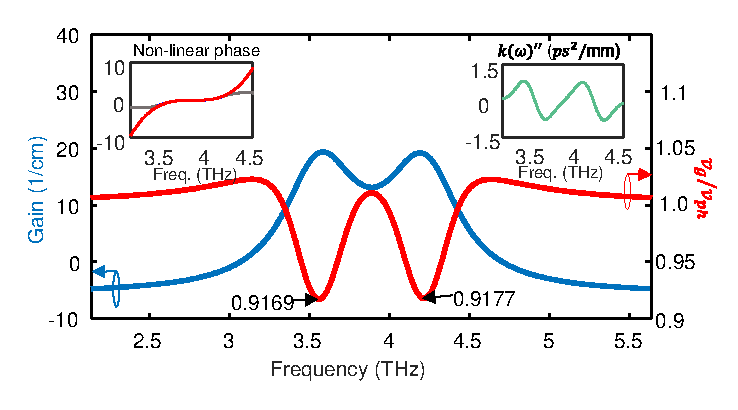
\includegraphics[scale=0.8]{img04_b.eps}
		\caption{Simulated spectral gain (blue curve, left y-axis) profile together with the normalized group velocity $v_{gr}/v_{ph}$ (red curve, right y-axis). (Left inset) The nonlinear phase acquired by the test pulse upon propagating for 2.5 mm inside the laser cavity. (Right inset) the second derivative of the wave number with respect to the angular frequency (in units of ps$^2$/mm) as a measure af GVD. }  \label{fig:img04}
	\end{center}	
\end{figure}
Even in the absence of bulk or waveguide dispersion, the doubly peaked resonant nature of the transition will contribute to a significant dispersion in the cavity which is expected to deteriorate the comb performance. Here a question naturally arises: "How does the presence of strong chromatic dispersion impact the mode proliferation process?". If the multimode behaviour of free running QCLs is due to four wave mixing (FWM), as already suggested in Ref. \cite{khurgin2014coherent}, then one would intuitively expect that such a high GVD violates the phase matching condition and thus yields this nonlinear process ineffective. However from experiment \cite{burghoff2014terahertz,rosch2015octave}, multimode operation of both mid-infrared and THz QCLs could be observed, even in the presence of strong dispersion. To investigate further this question we have to identify the nature of this mode generation mechanism and estimate the amount of phase mismatch induced by the resonant transition. 

\subsection{Four Wave Mixing}
\label{subsec:FWM}
We conducted numerical experiments, similar to the THz-TDs technique, where we pumped the ring cavity laser outlined above with two frequencies $\omega_1$ and $\omega_2 (< \omega_1)$. For 50 round trips we collected the signal and calculated the resulting power spectrum. Figures \ref{fig:img05}b,c and d illustrate the results from these simulations when the seed frequencies $\omega_1$ and $\omega_2$ were varied. In Fig. \ref{fig:img05}b, we chose $\omega_1$ and $\omega_2$ to be separated by the free spectral range, $\Delta\omega = 2\pi c/nL$, and to reside within the high frequency lobe of the spectrum. We can  clearly observe the formation of side-modes, separated by $\Delta \omega$, populating this whole frequency lobe. Similarly in Fig. \ref{fig:img05}c, our seed frequencies were chosen to be separated by $2\Delta \omega$ and again side-modes can be seen in the spectrum, however this time with mode spacing of $2\Delta \omega$. This kind of behaviour is a trademark for degenerate four wave mixing, i.e. the third order difference frequency generation \cite{butcher1991elements}, which is described by the susceptibility $\chi(-\omega_a; \omega_1,-\omega_2,\omega_1)$  and $\chi(-\omega_s; \omega_2,-\omega_1,\omega_2)$, where the frequency doubled pump frequencies $\omega_1$ and $\omega_2$ mix to produce side modes at the anti-Stokes $\omega_a$ and Stokes $\omega_s$ frequencies, respectively. This process is schematically illustrated in Fig. \ref{fig:img05}a.

\begin{figure}[h!]
	\begin{center}
		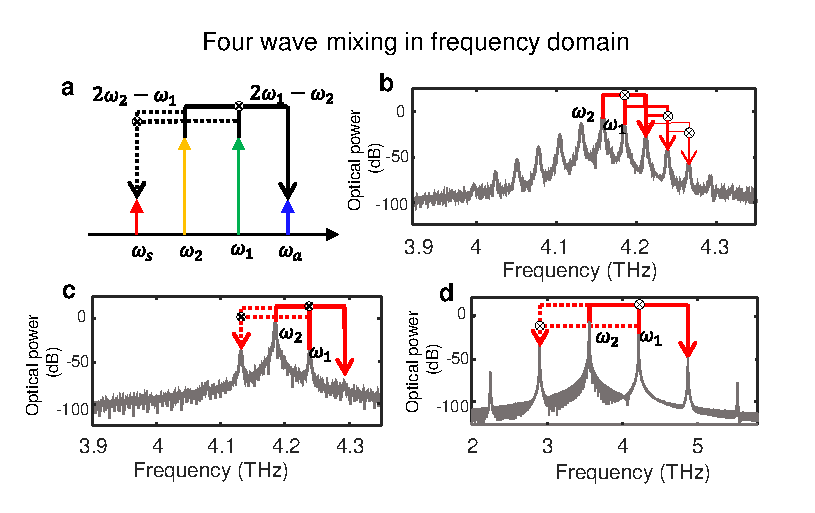
\includegraphics[scale=0.9]{img05_b.eps}
		\caption{\textbf{a}, Schematic representation of third order difference frequency generation \cite{butcher1991elements}, where two pump modes $\omega_1$,$\omega_2$ combine to produce sidebands at frequencies $\omega_a = 2\omega_1-\omega_2$ and $\omega_s=2\omega_2-\omega_1$. \textbf{b}, Optical spectrum obtained from THz-TDs simulations when the seed frequencies, $\omega_1$ and $\omega_2$, chosen to reside under the high frequency lobe part of the gain spectrum, were separated by the free spectral range $\Delta \omega$. \textbf{c}, Same as \textbf{b}, however this time $\omega_1-\omega_2 = 2\Delta \omega$. \textbf{d}, Optical spectrum from simulations where the seed frequencies were distributed under both peaks of the spectral gain.} \label{fig:img05} 
	\end{center}	
\end{figure}


We note that none of the modes under the low-frequency lobe part of the spectrum were activated in both experiments in Fig. \ref{fig:img05}b,c. The situation was equivalent when we pumped with $\omega_1,\omega_2$ distributed around 3.55 THz, i.e. we observed only mode proliferation around this frequency and no signal coming from the 4.21 THz lobe (not shown here). This means that in order for the four wave mixing process to start, some kind of seeding mechanism is necessary. Since in these experiments we considered a ring-cavity laser, multimode instabilities such as spatial hole burning \cite{gordon2008multimode} were not included and thus lasing in both spectral lobes failed to start, despite the comparable strengths of the gain. Lastly, Fig. \ref{fig:img05}d shows simulation results when both pump modes were chosen to be in resonance with the corresponding peaks of the gain. We again observe the familiar formation of side modes due to FWM.

The phase mismatch for this third order difference frequency generation process , depicted in Fig.\ref{fig:img05}a, is given by \cite{butcher1991elements}:
\begin{equation}
\Delta k L = \left [2k(\omega_1) - k(\omega_2)-k(\omega_a) \right ]L. 
\end{equation}
Taylor-expanding around $\omega_1$ up to third order in $\Delta \omega $, and taking that $\omega_2 = \omega_1 - \Delta \omega$ and $\omega_a = \omega_1 + \Delta \omega$ yields:
\begin{align}
\Delta k L & = L\Delta \omega^2 \left.\frac{\p^2 k}{\p \omega^2}\right|_{\omega_1} + O(\Delta \omega^4) \nonumber \\
		   &\approx \frac{1}{L}\times \left(\frac{\pi c}{n}\right)^2\times GVD(\omega_1),
\end{align}
for a Fabry-Perot laser. Plugging in typical values for $L = 5$ mm, $n=3.6$ and $GVD(\omega_1) \approx 2 $ ps$^2$/mm, we obtain a phase mismatch of $\Delta k L = 0.0274$ rad, which is negligible. This means that despite significant dispersion present in the cavity, under the favourable conditions of broadband gain, strong third order nonlinearity and some kind of multimode instability mechanism, such lasers can potentially emit a multitude of longitudinal modes, albeit each of them propagating with a different velocity. 

\subsection{Long time simulations of free running THz QCLs}
\label{subsec:tdsims}
In this subsection we present results from simulations over thousands of round trips of the device in Ref. \cite{burghoff2014terahertz}. Here we consider a Fabry-Perot cavity of length $L = 5 $ mm and a model parameter set, extracted with the aid of our Scrh�dinger-Poisson and Monte Carlo tools, when the bias was set at 11 kV/cm. To guarantee credibility of the computational results, selecting the time-propagation schemes for Eq. (\ref{eq:finalthreelevelmodel})  with the correct properties is of utmost importance, which is why, in Appendix \ref{sec:numerics}, we briefly discuss the numerical methods used throughout our simulations.
\begin{figure}[h!]
	\begin{center}
		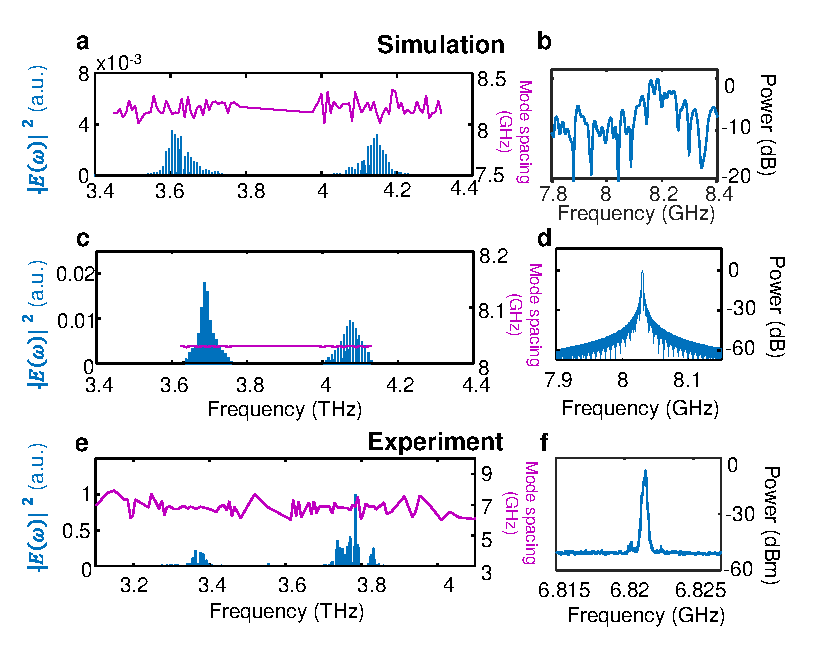
\includegraphics[scale=.9]{img06_b.eps}
		\caption{ Optical power spectra and beatnotes from simulations of the device from Ref. \cite{burghoff2014terahertz}, without dispersion compensation, \textbf{a} and \textbf{b}, with dispersion compensation, \textbf{c} and \textbf{d}, and the corresponding experimental measurements, \textbf{e} and \textbf{f}, at driving current of $0.9$ A. The right y-axis of \textbf{a}, \textbf{c} and \textbf{e} depicts the calculated spacing (in GHz) between all adjacent pairs above the noise threshold.} \label{fig:img06}
	\end{center}	
\end{figure}


In Fig. \ref{fig:img06}a-f, we compare the calculated spectra and beatnotes from simulations without dispersion compensation (Fig. \ref{fig:img06}a,b} and with dispersion compensation (Fig. \ref{fig:img06}c,d), to available experimental data \cite{burghoff2014terahertz} (Fig. \ref{fig:img06}e,f). In both the dispersion compensated and uncompensated case, we observe very good agreement with the detected optical power spectra (Fig. \ref{fig:img06}e), however substantial differences arise when we consider the corresponding beatnotes. Whereas experimental data shows a strong and narrow beatnote with a linewidth of approximately 0.5 MHz (Fig. \ref{fig:img06}\textbf{f}), in  Fig. \ref{fig:img06}b we observe a multi-beatnote signal distributed around 8.1 GHz. We attribute this behaviour namely to the slight differences of group velocity near the optical resonances (see Fig. \ref{fig:img04}), which probably results in the generation of sub-combs with different mode spacing. To investigate further, we computed the difference in position between each pair of adjacent peaks from the optical spectrum in Fig. \ref{fig:img06}a, and plotted the results on the right y-axis of Fig. \ref{fig:img06}a. We see that the free spectral range largely varies between 8.11 GHz and 8.15 GHz, which corresponds to the strongest peaks in the respective beatnote calculation, and supports our claim for the existence of multiple sub-combs propagating with different velocities. We can naturally extrapolate this deduction to situations where we have more complicated dispersion profile and more lasing modes in order to explain the formation of a chaotic beatnotes characteristic for incoherent multimode QCLs.   

Immediate comparison with experiment, Fig. \ref{fig:img06}e, shows us that the mode spacing of the real comb device varies very little around 6.8 GHz when the power of the spectral line is strong. This has been also confirmed from consequent SWIFT measurements in Ref. \cite{burghoff2015evaluating}, where the coherence of the comb lines is shown to approach unity when the signal to noise ratio is high. The variations in the mode-spacing of Fig. \ref{fig:img06}e, can be thus attributed to noise in the measurements as multi-beatnote behaviour cannot be observed in Fig. \ref{fig:img06}f.

\begin{figure}[h!]
	\begin{center}
		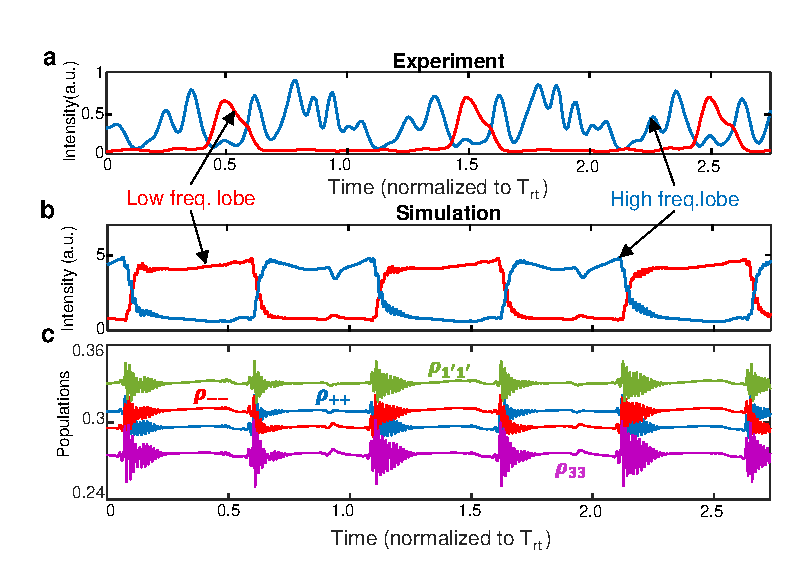
\includegraphics[scale=.95]{img08_b.eps}
		\caption{Insert caption here} \label{fig:img08}
	\end{center}	
\end{figure}

It is also interesting to observe that the line spacing in our simulation seems to alternate between 8.11 GHz and 8.149 GHz with a step of one longitudinal mode. Unfortunately, we have not been able to find an explanation for such a regime of operation and we also have failed to relate it to any existing experimental observations. 

The situation drastically changes when we employ dispersion compensation in our simulations. To cancel the accumulated nonlinear phase, during each iteration we Fourier-transform the envelope of the electric field and subtract from the resulting phasor a previously measured nonlinear phase component. We then inverse Fourier-transform the result before beginning the next iteration. In effect this approach emulates the application of a linear time-invariant filter onto the electric field signal, with a phase response equal to the "undesired" nonlinear phase, and an ideal, unity, magnitude response. The phase of the so implemented filter, centred around the carrier frequency of $3.88$ THz, is essentially the negative of $\Psi(\omega)$, depicted in the inset of Fig. \ref{fig:img04}. 

Again, the simulation was performed until steady state was reached and the resulting spectral power density and beatnote are plotted in Fig. \ref{fig:img06}c,d. We see that such a procedure equilibrates the difference in the group velocities of the high and low frequency lobe components of the gain, which results in producing an improved narrow (with FWHM linewidth limited by the DFT resolution) single beatnote. Consequent calculation of the mode-spacing (Fig. \ref{fig:img06}c right y-axis) shows very little variation of the distance between the adjacent comb lines, from where we can deduce that the simulation produced an almost perfect frequency comb. 




\section{Conclusion}
We have presented a theoretical method, based on the Maxwell-Bloch equations, suitable for efficient time domain simulations of terahertz quantum cascade lasers. We applied our model to characterize different regimes of operation of a well known resonant phonon THz QCL \cite{burghoff2014terahertz}, and showed how the fairly complicated dynamics between four wave mixing, chromatic dispersion and multimode instabilities, such as spatial hole burning, are at play in such a device. Based on our results, we can confidently outline the essential ingredients for such a laser to emit a stable and coherent frequency comb. Those are namely:
\begin{enumerate}
	\item the existence of an instability that will seed the multimode dynamics,
	\item the presence of a strong third order nonlinearity for efficient mode proliferation,
	\item the correct compensation or lack thereof dispersion, as to ensure that the majority of lasing modes propagate with the same group velocity.  
\end{enumerate}
Furthermore, we identified the type of four wave mixing responsible for the multimode spectra, and came to the conclusion that despite the presence of a significant group velocity dispersion, the process will remain efficient due to strongly reduced phase mismatch (especially for devices with longer cavity). 

As a future outlook, it will be interesting to use our model to characterize and quantify the amount of noise present in the electric field, evaluate the effect of different model parameters onto the emitted modes' linewidth and estimate the ultimate limit to which it can converge.

\begin{appendices}
	\section{Numerics}
	\label{sec:numerics}
	
	Equations (\ref{eq:finalthreelevelmodel}) comprise a system of two partial and fourteen ordinary differential equations. As there is no general analytical solution of Eq. (\ref{eq:finalthreelevelmodel}), we time step the latter numerically with the aid of carefully chosen schemes. 
	
	The field propagation equations, Eq. (\ref{eq:rtwave}), are a pair of inhomogeneous hyperbolic equations the accurate numerical solution of which is far from trivial. From the area of computational fluid dynamics \cite{wesseling2009principles}, it is known that a simple central differences discretization scheme for Eq. (\ref{eq:rtwave}) will be highly unstable due to the introduction of strong \emph{numerical} dispersion near sharp edges or discontinuities of the solution. A finite difference scheme that does not generate such spurious oscillations is called monotonicity preserving \cite{wesseling2009principles} and its usage is essential for the correct interpretation of simulation results, especially when one tries to quantify the amount of \emph{physical} dispersion present. Without getting too much into detail, we present a second order linear finite difference discretization scheme, possessing the monotonicity preserving property (in the case when $f_\pm \propto E_\pm$),  for the model equation:
	\begin{equation}
	\label{eq:genericwave}
	\frac{\partial E_{\pm}}{\partial t}  = \mp c\frac{\partial E_{\pm} }{\partial x} +f_{\pm}(x,t) + k E_{\pm}.
	\end{equation}
	Let us take an equidistant spatio-temporal grid with grid size $\Delta x$ and time step $\Delta t$ for our discretization and let us denote the value of the grid variables at spatial point $x_m=m \Delta x $  and at time $t_n = n\Delta t$ as $E_{\pm}(m,n)$. Then the time stepping scheme we use is based on a second order upwind discretization, first introduced by Risken and Nummedal \cite{risken1968self}, and is given by
	\begin{align}
	\label{eq:riskennummedal}
	E_{\pm}(m,n+1) &= E_{\pm}(m \mp 1,n) + \Delta t \big ( f_{\pm}(m,n) +k E_{\pm}(m,n) \big ) \nonumber \\ 
	& + \frac{\Delta t^2} {2} \Bigg ( \left [  \frac{\partial f_{\pm} }{\partial t} \right]_m^n \mp  c \left [  \frac{\partial f_{\pm} }{\partial x} \right]_m^n 
	\mp 2kc \left[ \frac{\partial E_{\pm} }{\partial x} \right]_m^n  + kf(m,n) + k^2 E_{\pm} (m,n) \Bigg ),
	\end{align} 
	where time step is chosen as $\Delta t = \Delta x n/c$, with $c/n$ the velocity of light in the medium. The evaluation of the time derivative of $f(t,x)$ can be computed analytically from the density matrix equations as $\p f_{\pm}/\p t \propto \p \eta_{32}^{\pm}/\p t$. As for the other terms in rectangular brackets, $\left [ \partial f_{\pm} /\partial x \right]_m^n$ and  $\left[ \partial E_{\pm}/\partial x \right]_m^n$, those can be computed via forward/backward finite differences, depending on the propagation direction of the field. 
	
	Lastly, it is worthwhile to note that this numerical scheme, in apparent violation of Godunov's barrier theorem \cite{godunov1959difference}, is indeed linear, second order accurate and monotonicity preserving. The reason for that is namely because we have imposed the magic time step in our time propagation. 
	
	As for the density matrix equations, Eq. (\ref{eq:rho11-dm}-\ref{eq:rho12-dm}), they form a system of ordinary differential equations and the usage of any out of the box numerical solver ought to suffice. In our experience a suitable method which is high-order accurate and also preserves the normalization property of the density matrix, i.e. $\Tr(\rho) = 1$, is given by the fifth order linear multi-step Adams-Bashforth method, calculating the update of the time dependent variable as a linear combination of several past time-steps
	\begin{equation}
	\label{eq:adams-bashforth}
	y^{n+1} = y^{n} + \Delta t \sum\limits_{m = 0}^{k-1} c_m f(t_{n-m},y_{n-m}) \text{	,}
	\end{equation}
	where again we have assumed the model equation:
	\begin{equation}
	\label{eq:adams-bashforth-model}
	\dot{y}(t) =f(t,y).
	\end{equation}

	\section{Simulation parameters}
	\label{sec:params}
	In the following table we summarize the parameter set used for our simulations, where we have endeavoured to keep the amount of phenomenologically included values to a minimum. Therefore the only empirically included values are essentially the pure dephasing times  $\tau_{32}^{pure},  \tau_{1'2}^{pure} $ and $\tau_{1'3}^{pure}$. For the former two parameters, we have set the value to $1.25$ ps which was chosen to correspond to the observed spectrum's full width at half maximum, whereas the latter was set to $0.4$ ps, modelled after Ref. \cite{dupont2010simplified}.
	\begin{table}[H]
		\centering
		\footnotesize
		\begin{tabular}{ p{35 mm} c c}	
			\hline
			\textbf{Parameter}  & \textbf{Symbol} & \textbf{Value}\\
			\hline
			Avg. carrier density & N & 5.6$\times10^{15}$ (cm$^{-3}$)  \\
			Overlap factor & $\Gamma$ & 0.8 \\
			Linear amplitude loss coeff. & $l_0$ & 10 (cm$^{-1}$) \\
			Dipole matrix element &$\mu_{32}$& 4.0 (nm) $\times |e|$  \\
			Refractive index  & $n$ & 3.6 \\
			Diffusion constant & D & 46 (cm$^2$/sec)\\
			Left/right mirror reflectivity & $ R_{L/R} $ & 1.0 \\
			1'$\rightarrow$3 pure deph. time & $\tau_{1'3}^{pure}$ & 0.4 (ps)\\
			3 $\rightarrow$2 pure deph. time & $\tau_{32}^{pure}$ & 1.25 (ps)\\
			1'$\rightarrow$2 pure deph. time & $\tau_{1'2}^{pure}$ & 1.25 (ps)\\
			3 $\leftrightarrow$ 2 resonance energy & $ \Delta_{32}$ &  16.1 meV\\
			1'$\leftrightarrow$ 3 detuning energy & $\Delta_{1'3} $ &  0.0198 meV\\
			1'$\leftrightarrow$ 3 anticrossing energy & $\hbar\Omega_{1'3}$ &  -1.38 meV\\
			\hline 
		\end{tabular}
		\caption[Table caption text]{ Simulation parameters for a ring cavity THz QCL, modelled after the device in Ref. \cite{burghoff2014terahertz}.}
		\label{tab:table01}
	\end{table}
We have also calculated, with the aid of an ensemble Monte Carlo simulation code \cite{jirauschek2014modeling}, the scattering rates between each pair of subbands of the active region treated in Sec. \ref{sec:application}. The code includes all relevant scattering mechanisms reported to play a role in quantum cascade lasers, and those are: longitudinal and transverse optical phonons, acoustic phonons, interface roughtness and impurity scattering as well as many body effects such as electron-electron scattering. The calculated rates are present in units of THz and are summarized in the matrix below.
\begin{table}[H]
	\centering
	\footnotesize
	\begin{tabular}{ r | c c c c c c c}	
	\hline
 & \textbf{INJ1}  & 	\textbf{INJ2}& 	\textbf{ULL} & 	\textbf{LLL1} & 	\textbf{LLL2} & 	\textbf{DEP1} & 	\textbf{DEP2}\\
	\hline
 \textbf{INJ1}  &	0.0000 & 0.7828  &  0.0177  & 0.0013  & 0.0006 &  0.0020 &  0.0020 \\
 \textbf{INJ2}  &   0.4955 & 0.0000  &  0.0667  & 0.0018  & 0.0007 &  0.0018 &  0.0020  \\
 \textbf{ULL}  &    0.0365 & 0.1216  &  0.0000  & 0.1328  & 0.1024 &  0.0492 &  0.0437  \\
 \textbf{LLL1}  &   0.0241 & 0.0279  &  0.0774  & 0.0000  & 0.4674 &  0.7713 &  0.5534 \\
 \textbf{LLL2}  &	0.0119 & 0.0195  &  0.0309  & 0.2750  & 0.0000 &  1.0693 &  1.1260 \\ 
 \textbf{DEP1}  &  0.0019 & 0.0029  &  0.0031  & 0.0037  & 0.0055 &  0.0000 &  0.7828  \\
 \textbf{DEP2}  &	0.0012 & 0.0017  &  0.0019  & 0.0014  & 0.0045 &  0.4856 &  0.0000 \\
	\hline 
	\end{tabular}
	\caption[Table caption text]{ Total scattering rates between each pair of relevant subbands of the device in Ref. \cite{burghoff2014terahertz}, calculated within the tight-binding approximation with 
		our ensemble Monte Carlo code. The rates are presented in THz and the diagonal elements are set to zero as they will depend on the periodic boundary conditions employed.}
	\label{tab:table02}
\end{table}

	
	
\end{appendices}

\end{document}
